\documentclass{my_cv}
%\usepackage{showframe}

\usepackage[danish]{babel} 
\usepackage[utf8]{inputenc}


%\usepackage[applemac]{inputenc}

\begin{document}
\firstpagestyle{\contact{Engvej 251}{9440 Aabybro}{privat@jossound.dk}{40158236}}
%
\noindent
\begin{minipage}[t]{.69\textwidth}%
    \vspace*{4pt}
    \name{Jonas Flensborg Riis Buchholdt - CV}
	\degree{Cand. Polyt. i akustik og signalbehandling}
	%
    \section{Resumé}
    %\vspace{4pt}
    Som uddannet Cand. Polyt. i akustik og signalbehandling ser jeg mig som en stærk kandidat til jobbet inden for hardware til lyd. Jeg har arbejdet med DSP og optimering af kode via assembly. Jeg har konstrueret højttalere ud fra fundne parameter for enheder. Jeg har altid interesseret mig for, at designe forstærkere og højttalere. Mit master projekt gik ud på, at skabe et jævnt lydtryk, og ensartet frekvens respons i bevægende atmosfæriske tilstande. Grundet min store interesse inden for emnet, har jeg opbygget et udlejnings- og akustik rådgivningsfirma under mine studier. Dette har givet mig rigtig mange erfaringer omkring, hvordan folk oplever selve lyden, og hvad der skal til for, at folk får en god lydoplevelse.

\end{minipage}
\hfill%
\begin{minipage}[t][0.3\textwidth][b]{.29\textwidth}
	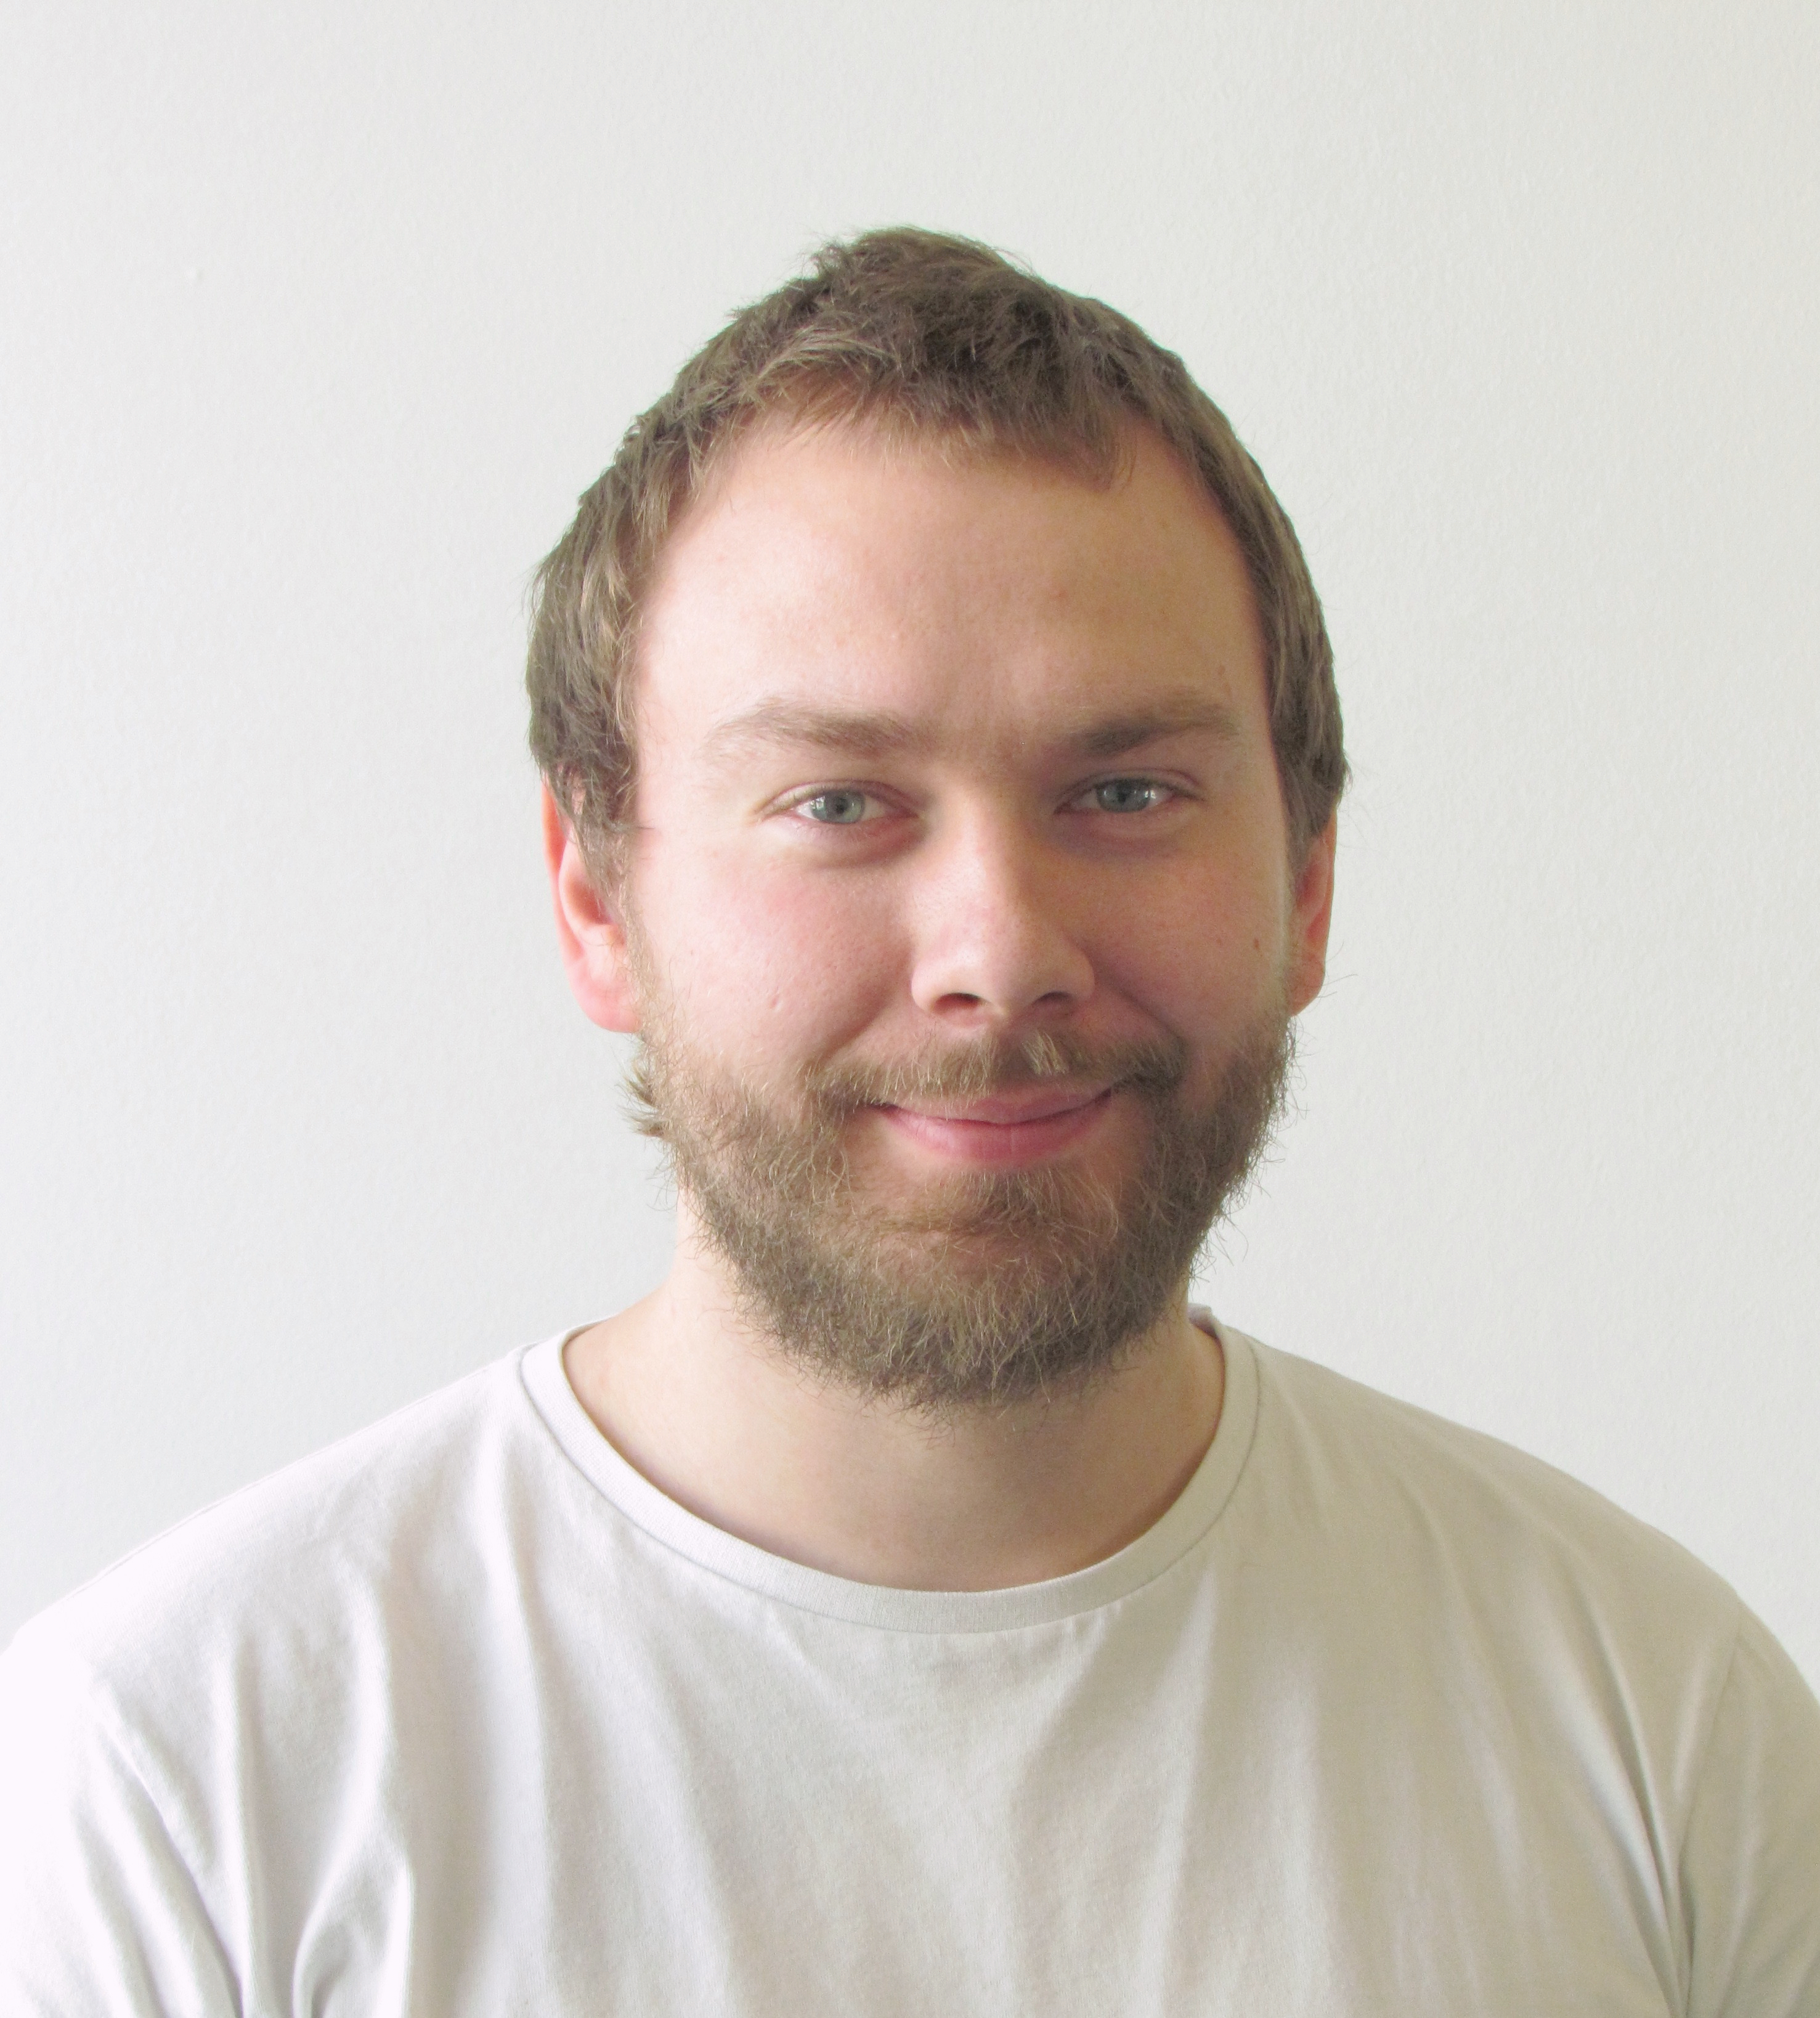
\includegraphics[width=\textwidth]{figures/mig.jpg}
\end{minipage}%
%
\section{Uddannelse}
\datedsubsection{2017--2019}{Civilingeniør i akustik og signalbehandling (AAU)}
%
\begin{focusTable}
	& Forskning og udvikling inden for hardware, akustik og audio industrien.\\
	& Gruppearbejder, struktureret tværfagligt samarbejde og selvstændigt.\\
	& Tage ansvar for egen professionel udvikling og specialisering.
\end{focusTable}
%
\project{10}{Adaptiv optimering af lyddækningen i bevægelig atmosfære}
\begin{projectTable}
	Metode(r) 	& Teori indenfor lydens udbredelse i bevægelig atmosfære \\
				& Impulsrespons via statistisk tids synkronoseret sine sweep målinger\\
				& Affoldning i frekvensdomænet\\
				& Programmering af måleprogram i MATLAB\\
				& Signal processering i Matlab\\
				& Akustiske målinger i lyddøt rum, i vindtunnel og udendørs. 
\end{projectTable}
%
\project{9}{inteligibility differenses mellem airborn og bone born lyd.}
\begin{projectTable}
	Metode(r)	& Måling af psykometrisk funktion på testpersoner\\
				& Hint metoden\\
				& Programmering af test signal i Matlab\\
				& Programmering af estimeringsfunktioner i Matlab
\end{projectTable}
%
\project{8}{Optimering af FIR filter til directionaliteten på cardioid low frequency højtaler.}
\begin{projectTable}
	Metode(r)	& Måling og modulering af givet transducere.\\
				& Design og konstruktion at kabinet.\\
				& Design og Programmering af genetiske algoritmer.\\
				& Design a test i lyddøt rum.\\
\end{projectTable}
%
\project{7}{Statistisk Identificering af alarmer}
\begin{projectTable}
	Metode(r) 	& Statistiske korrelation metoder til Identificering as periodiske signaler.\\
				& Måling af alarmer in støjende omgivelser.\\
				& Programmering af test i Matlab
\end{projectTable}
%
\datedsubsection{2012--2015}{Bachelor i Elektronik og IT (AAU)}
\begin{focusTable}
				& Analog og digital elektronik.\\
				& Udvikling af software, herunder samspil med hardware.\\
				& Metoder og redskaber til at beskrive, analysere, modellere, implementere, teste og dokumentere elektroniske systemer på et videnskabeligt grundlag.\\
				& Teorier og metoder, der indgår i indlejrede realtids signalbehandlingssystemer.
\end{focusTable}
%
\project{6}{Guitar effekter}
\begin{projectTable}
	Metode(r)	& DSP\\
				& Assembler med både single og dobel præsition\\
				& Realtid processering
\end{projectTable}
%
\project{5}{Autonom grasslåmaskine styret ad differentiale GPS}
\begin{projectTable}
	Metode(r)	& Mikroprocessor\\
				& FPGA programmering\\
				& GPS signaler\\
				& Wi-Fi
\end{projectTable}
%
\project{4}{Kelvin kontrold af LED array besseret på lyset udefra}
\begin{projectTable}
	Metode(r)	& FPGA\\
				& whdl\\
				& C\\
				& Design af eksterne hardware moduler\\
				& Konstruktion af hardware med ætseteknik
\end{projectTable}
%
\project{3}{Klasse H forstærker}
\begin{projectTable}
	Metode(r)	& Strømspejl\\
				& Complementary effekt opkobling til at opnå højere outputspænding\\
				& Vbe multiplier\\
				& Konstantstrømsgenerator\\
				& Lydsignalsstyret strømforsyning som følger output signalet\\
				& Tilbagekobling\\
				& Analog filtre\\
				& Design af hardware\\
				& Simulering af hardware		
\end{projectTable}
%
\project{2}{Lokaliseringsenhed ved hjælp af lyd}
\begin{projectTable}
	Metode(r)	& Mikroprocessor\\
				& tidsdiference ved lydsignaler\\
				& C programmering\\
				& Aktuatorstyring\\
				& Arduino mega modul
\end{projectTable}
%
\project{1}{Elektronisk nødstop på roterende værktøj}
\begin{projectTable}
	Metode(r)	& Mikroprocessor\\
				& accelerometer og gyro\\
				& C programmering\\
				& Hardware design\\
				& PCB
\end{projectTable}
%
\datedsubsection{2012--2015}{Elektronik fagtekniker  (EUC syd) ved LINAK A/S}
\begin{focusTable}
				& Analog og digital elektronik.\\
				& HF kredsløb.\\
				& Forsærker, SMPS og linear strømforsynings kredsløb.\\
				& Fejlfinding af hardware.\\
				& Metoder til test og beregning af grundlæggende elektronik.\\
\end{focusTable}
%
\section{Erhvervserfaring}
\datedsubsection{2009--2013}{Elektronik fagtekniker, Lærling ved LINAK A/S}
\begin{itemize}
	\item Lager optimering 
	\item Fejlfinding på elektronik
	\item Design af elektronik
\end{itemize}
%
\datedsubsection{2009--2019}{Akustik rådgiver, Ejer af Jossound}
\begin{itemize}
	\item Udlejning af lyd
	\item Rådgivning inden for lyd
	\item Akustisk rådgivning inden for lyd
\end{itemize}
%
\datedsubsection{2019--2019}{Rådgiver ved RTX i focusgruppe}
\begin{itemize}
	\item Rådgivning omkring sammenspil blandt elektronik og brug af elektronik i tidspressede siturationer.
	\item Metoder til bedre design af funktionaliteten af trådløse systemer til PA og musik instrumenter.
\end{itemize}
%
\section{Sprog}
\begin{tabular}{l}
	\skill{Dansk}{5} \\
	\skill{Engelsk}{5} \\
	\skill{Tysk}{2}
\end{tabular}
%
\section{IT}
%
\newlength{\columnWidth}
\setlength{\columnWidth}{\dimexpr(\textwidth/3)\relax}
\begin{tabular}{p{\columnWidth} p{\columnWidth} p{\columnWidth}}
	\skill{Python}{4} 	& \skill{SketchUp}{3}	& \skill{Word}{5} 		\\
	\skill{Matlab}{5}	& \skill{Fusion360}{3}	& \skill{Excel}{5}		\\
	\skill{C}{4}		& \skill{OrCad}{2}		& \skill{powerpoint}{5} \\
	\skill{Assembler}{4}& \skill{Altium}{2}		& \skill{Latex}{5}		\\
	\skill{WHDL}{3}		& \skill{LT Spice}{4}	&						\\
	\skill{Processing}{3}&						&	
\end{tabular}
%
\section{Personlig}
Jeg er bosat i Aabybro sammen med min kone. Mine fritidsinteresser er gymanstik, sport og powertumbling, musik og koncerter både som audience og lydinginør ved pulten. .
Jeg bor i Nørhalne tæt ved Aabybro i Nordjylland sammen med min kone Heidi. Vi ejer en gård som vi renoverer løbende på. Vi har bil, så arbejde i det nordlige jylland passer godt geografisk. Det meste af min tid går med arbejde af lyd. det er det jeg virkelig brænder for. Mit studie og projekter er basseret på lyd, min fritid er basseret på lyd men samtidig sætter jeg familien højt. vi kan godt lide at rejse og tage på ture. Vi har dyr, både hund og katte. Jeg har derudover altid interreseret mig for gymnastik, og har gået til springgymnastik og powertumbling siden jeg var 8 år. 

%	
\end{document}
